\section{ENABLING TECHNOLOGIES, APPLICATION REQUIREMENTS, AND 6G NETWORK EVIDENCE}
\label{sec:technologies_applications_6g}
Validation shows how far a reported system was tested. We now follow the
technologies that form communication and sensing observables into application
requirements and 6G network roles. Because a study may contribute to several
technology and application labels, their counts describe coverage within the
corpus.

Figure~\ref{fig:technology_application_chain} follows this evidence chain from
optical generation and transport through waveform formation, spatial control,
inference, selected application domains, and 6G network positioning.

\begin{figure*}[!t]
\centering
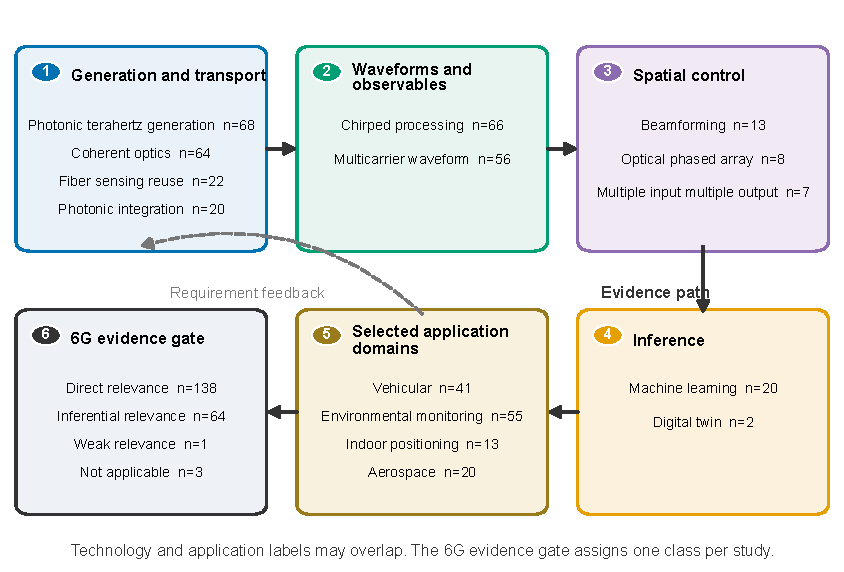
\includegraphics[width=\textwidth]{figures/final_submission_2026-08-25/fig08_technology_application_chain.pdf}
\caption{Organization across system layers of the mechanisms that create and shape
O-ISAC observables and connect them to service requirements. Technology and
application counts describe overlapping corpus coverage, so a study may
contribute to several displayed categories. The 6G evidence gate is exclusive
and assigns each of the 206 studies to one relevance class. Selected application
domains illustrate the requirement flow, while Table~\ref{tab:application_requirements}
provides the complete application inventory.}
\label{fig:technology_application_chain}
\end{figure*}

The chain shows that network interpretation depends on continuity across the
physical observable, the joint design choice, the application condition, and
the reported network role. The displayed categories guide the reader through
that relationship, while the following subsections retain the platform
conditions and study evidence.

\subsection{Technologies That Create and Shape Observables}

The main technology labels occupy complementary points in the signal chain.
Photonic generation creates or translates the carrier. Chirped processing maps
delay or motion to beat frequency. Coherent reception preserves phase, and OFDM
provides controllable time and frequency resources. A single architecture can
combine several of these mechanisms.

OFDM supports joint operation by placing payload and sensing resources within
one signal structure. The sensing observable may come from pilots, payload
tones, cyclic prefixes, reserved subcarriers, or a dedicated processing branch.
This choice determines which samples are known at the receiver and how
interference enters the estimate. Optical modulation constraints and the
measurement plane used for SNR shape the interpretation. Embedded pilot fiber
sensing and indoor optical positioning show how the same multicarrier principle
serves different observables and geometries
\cite{OISAC_SCR00007,OISAC_SCR01024}.

Chirped and coherent systems draw on phase continuity and a shared timing
reference. A returned chirp can reveal range or motion as the transmitted signal
carries data. A coherent front end preserves small phase changes for distributed
sensing and demodulation. Photonic generation can extend the reference to
wideband millimeter wave or terahertz carriers. Full photonic dechirping and
coherent fiber vibration sensing illustrate these two uses
\cite{OISAC_SCR01000,OISAC_SCR00647}. Their performance depends on laser
stability, reference distribution, conversion efficiency, receiver bandwidth,
and calibration.

The optical stage governs carrier generation and reference stability. Once the
carrier is radiated, the communication and sensing paths follow microwave,
millimeter wave, or terahertz propagation. In a free space optical link, the
optical beam itself traverses the channel. System evaluation should therefore
follow the signal across both physical domains and identify where power, SNR,
bandwidth, and timing are measured. This view makes the interface between
components part of the joint system.

Spatial control changes both the communication link budget and the sensing
geometry. Beamforming, optical phased arrays, multiple input multiple output
processing, and reconfigurable optical intelligent surfaces provide different
forms of spatial control. Beamforming directs energy. An optical phased array
provides one steering mechanism. Multiple input multiple output processing uses
several spatial dimensions, and an intelligent surface reshapes an intermediate
propagation boundary. A system may combine these roles.

A narrow beam improves received power and angular selectivity while making
acquisition, tracking, blockage, and calibration central to joint performance.
The joint use of an optical phased array and OFDM and the use of frequency comb
beamforming connect steering with ranging or imaging
\cite{OISAC_SCR00941,OISAC_SCR00362}. Multiple input multiple output processing
adds communication streams, sensing diversity, or separation among targets and
paths. Structured fields and hybrid systems that combine free space
optics with fiber Bragg gratings place these spatial dimensions at different
points in the architecture \cite{OISAC_SCR00268,OISAC_SCR00277}. Meaningful
comparison therefore requires the independent dimensions, geometry, and
calibration method.

The intelligent surface evidence consists of one study that models a mobile
free space optical path controlled by an optical intelligent surface
\cite{OISAC_SCR00914}. A separate laboratory demonstration uses mechanically
rotated Risley prisms to steer a photonically generated terahertz signal
\cite{OISAC_SCR00953}. Both mechanisms redirect energy, and each uses different
surface physics, propagation laws, control variables, and validation settings.
Their separate treatment preserves the physical meaning and provides two
starting points for broader experimental comparison.

\subsection{Integration Beyond the Waveform}

Integration and inference move joint design beyond waveform selection.
Photonic integration appears in 20 studies, fiber distributed acoustic sensing
in 22, and machine learning or artificial intelligence in 20. Two studies use
digital twins. A further 19 studies contain specialized mechanisms grouped as
other because they fall outside the broad technology labels. Together, these
categories cover device integration, infrastructure reuse, inference, and a
diverse long tail.

Photonic integration can place generation, reference distribution, beam
control, and detection on a compact hardware path. This arrangement reduces
duplicated paths and brings packaging, thermal drift, crosstalk, and calibration
into the same design problem. Microcomb synchronization coordinates wireless
data with radar imaging. A distributed W band system uses radar estimates for
beam alignment and flexible data service
\cite{OISAC_SCR00406,OISAC_SCR00502}. Both examples show how a shared reference
can connect communication and sensing hardware.

Fiber distributed acoustic sensing follows a complementary route by using the
transmission medium as a spatial sensor. Phase, backscatter, and polarization
can reveal events along the route as the fiber carries traffic. Coherent
multicore transmission with distributed sensing and operational submarine cable
monitoring illustrate two scales of this infrastructure reuse
\cite{OISAC_SCR00346,OISAC_SCR00957}. The central design question becomes how to
preserve the optical observable together with traffic continuity.

Learning turns optical observations into event labels, positions, field
estimates, channel predictions, and resource decisions. Each task is best read
with its definition, reference data, training distribution, evaluation shift,
uncertainty, and inference cost. Fiber diagnosis, federated visible light
positioning, and wearable optical sensing show the range from distributed
infrastructure to personal use
\cite{OISAC_SCR01006,OISAC_SCR01081,OISAC_SCR00376}.

A neural network can also take part in both functions. In one coherent link,
the model compensates transmission impairments and estimates distributed power
and abnormal loss \cite{OISAC_SCR00949}. The two outputs share the link while
retaining separate targets and reference data. Digital twins add another model
layer. One represents vehicular edge resources, and another provides a model
aided physical reference for coherent fiber sensing
\cite{OISAC_SCR01059,OISAC_SCR01185}. Clear reporting of the represented state,
update process, mismatch model, and resulting decision gives these models an
explicit system role.

\subsection{Applications as Operating Requirements}

Applications translate the mechanisms above into conditions that a joint
service must satisfy. Table~\ref{tab:application_requirements} retains all
thirteen application domains and maps each one to its joint role and defining
evaluation conditions. A fiber platform for vehicles, for
example, carries data at high rates and measures distributed temperature
\cite{OISAC_SCR00123}. Devices used by people connect communication or remote
alerts with motion, falls, air pressure, physiology, or gesture
\cite{OISAC_SCR00451,OISAC_SCR00294,OISAC_SCR00376}. Each application therefore
changes what the experiment must demonstrate, even when both functions share
the same optical interface.

\begin{table*}[!t]
\caption{Application domains and operating requirements in the reviewed corpus}
\label{tab:application_requirements}
\centering
\footnotesize
\setlength{\tabcolsep}{3pt}
\renewcommand{\arraystretch}{1.05}
\begin{tabularx}{\textwidth}{@{}
>{\raggedright\arraybackslash}p{0.16\textwidth}
>{\raggedright\arraybackslash}p{0.39\textwidth}
>{\raggedright\arraybackslash}X
>{\centering\arraybackslash}p{0.095\textwidth}@{}}
\toprule
\multicolumn{4}{@{}l}{\emph{Network and mobility}} \\
\addlinespace[1pt]
\textbf{Domain, n (\%)} & \textbf{Common communication and sensing role} &
\textbf{Key operating condition} & \textbf{Studies} \\
\midrule
\textbf{6G and access} 100 (48.5\%) & Access and transport with channel, target,
position, or environment sensing & Timing, orchestration, continuity, and
evidence for both functions & \cite{OISAC_SCR00277,OISAC_SCR01049} \\
\addlinespace[1.25pt]
\textbf{Vehicular} 41 (19.9\%) & Vehicle data links with range, motion, pose,
temperature, or channel sensing & Changing geometry, acquisition, tracking, and
service continuity & \cite{OISAC_SCR00123,OISAC_SCR00273} \\
\addlinespace[1.25pt]
\textbf{Optical access} 32 (15.5\%) & Access and transport links with channel,
event, or fiber state sensing & Reach, synchronization, and traffic continuity &
\cite{OISAC_SCR00007,OISAC_SCR01006,OISAC_SCR01049} \\
\addlinespace[1.25pt]
\textbf{Indoor positioning} 13 (6.3\%) & Indoor optical links with user or robot
position and orientation sensing & Geometry, calibration, coverage, and update
continuity &
\cite{OISAC_SCR00910,OISAC_SCR01024} \\
\addlinespace[1.25pt]
\textbf{Data center} 4 (1.9\%) & Short reach data links with channel estimation
or link state sensing & Traffic continuity and calibrated link references &
\cite{OISAC_SCR00007} \\
\bottomrule
\end{tabularx}

\vspace{3pt}
\begin{tabularx}{\textwidth}{@{}
>{\raggedright\arraybackslash}p{0.16\textwidth}
>{\raggedright\arraybackslash}p{0.39\textwidth}
>{\raggedright\arraybackslash}X
>{\centering\arraybackslash}p{0.095\textwidth}@{}}
\toprule
\multicolumn{4}{@{}l}{\emph{Infrastructure}} \\
\addlinespace[1pt]
\textbf{Domain, n (\%)} & \textbf{Common communication and sensing role} &
\textbf{Key operating condition} & \textbf{Studies} \\
\midrule
\textbf{Environmental monitoring} 55 (26.7\%) & Distributed links with vibration,
temperature, or environmental event sensing & Persistent observation,
localization, and traceable reference data &
\cite{OISAC_SCR00957,OISAC_SCR01006,OISAC_SCR01095} \\
\addlinespace[1.25pt]
\textbf{Smart infrastructure} 41 (19.9\%) & Infrastructure links with structural,
motion, or event monitoring & Continuous observation, calibration, and
resilient alert delivery & \cite{OISAC_SCR00277,OISAC_SCR00763,OISAC_SCR01006} \\
\addlinespace[1.25pt]
\textbf{Industrial} 34 (16.5\%) & Industrial data or control with process,
strain, temperature, motion, or position sensing & Delay, continuity,
calibration, and safe operation & \cite{OISAC_SCR00277,OISAC_SCR00376} \\
\addlinespace[1.25pt]
\textbf{Security and surveillance} 26 (12.6\%) & Monitoring links with anomaly,
event, or location sensing & Coverage, event discrimination, and alert latency &
\cite{OISAC_SCR01006} \\
\bottomrule
\end{tabularx}

\vspace{3pt}
\begin{tabularx}{\textwidth}{@{}
>{\raggedright\arraybackslash}p{0.16\textwidth}
>{\raggedright\arraybackslash}p{0.39\textwidth}
>{\raggedright\arraybackslash}X
>{\centering\arraybackslash}p{0.095\textwidth}@{}}
\toprule
\multicolumn{4}{@{}l}{\emph{Human use, extreme settings, and remaining domains}} \\
\addlinespace[1pt]
\textbf{Domain, n (\%)} & \textbf{Common communication and sensing role} &
\textbf{Key operating condition} & \textbf{Studies} \\
\midrule
\textbf{Healthcare} 6 (2.9\%) & Wearable or ambient links with vital sign,
activity, or gesture sensing & Motion robustness, physiological reference,
illumination, and user safety & \cite{OISAC_SCR00001,OISAC_SCR00376} \\
\addlinespace[1.25pt]
\textbf{Aerospace} 20 (9.7\%) & Satellite links with atmospheric or wavefront
sensing & Pointing, turbulence, delay, and link adaptation &
\cite{OISAC_SCR00456} \\
\addlinespace[1.25pt]
\textbf{Underwater} 2 (1.0\%) & Underwater link concepts and subsea data links
with temperature or event sensing & Water attenuation or cable calibration,
packaging, and access & \cite{OISAC_SCR00763,OISAC_SCR01095} \\
\addlinespace[1.25pt]
\textbf{Other} 17 (8.3\%) & Emerging links with range, imaging, object, or
channel sensing & Metrics and reporting specific to the task & \cite{OISAC_SCR00953} \\
\bottomrule
\end{tabularx}
\vspace{1pt}
\parbox{\textwidth}{\raggedright\footnotesize\emph{Note.} Application domains
overlap, so a study may contribute to more than one row. Counts and percentages
describe coverage within the 206 included studies. For each domain, the table
includes a selected study set and lists the corresponding references in the
final column. The 6G and access row identifies the application category, and
the final subsection provides the 6G relevance classification.\par}
\end{table*}

Across the map, the dominant requirement moves with the application. Network
and mobility settings emphasize acquisition, timing, and continuity. Deployed
infrastructure emphasizes persistent observation alongside carried traffic.
Human use and extreme settings add physiological references, safety,
privacy, pointing, atmosphere, packaging, and access to the test environment.
These requirement bundles show which operating conditions must accompany a
reported result before it can support comparison or reuse.

\subsection{From 6G Relevance to Network Evidence}

The 6G relevance gate in Figure~\ref{fig:technology_application_chain} assigns
each study one corpus position. Direct cases connect the reported system
explicitly to a 6G role, as illustrated
by \cite{OISAC_SCR00362,OISAC_SCR01049}. Inferential cases contribute an
enabling link that gains meaning from additional network context, as illustrated
by \cite{OISAC_SCR00007,OISAC_SCR00647}. The remaining classes capture a lighter
connection to 6G or an application focus outside that framing, as illustrated
by \cite{OISAC_SCR00959,OISAC_SCR00294}.

The distribution connects the reviewed corpus with 6G access, transport,
localization, automation, environmental awareness, and generation of carriers
at high frequencies. A relevance code therefore locates a study within the 6G
discussion. Standard conformance, interoperability, and deployment readiness
require additional evidence tied to the relevant network framework
\cite{ITUR_M2160_2023}.

A stronger network interpretation emerges when the optical or photonic
subsystem occupies an explicit role across the complete network path. Access, fronthaul, transport,
edge processing, and service control bring timing, mobility, orchestration,
energy, security, and recovery requirements. Evidence at this level evaluates
useful communication and sensing under the conditions of that role and reports
the resources needed to sustain both. This creates a traceable path from the
physical observable and hardware to the service objective.

Within this survey, 6G relevance is strongest when both functional outcomes and
their operating conditions remain traceable to a network role. The resulting
evidence chain links physical observables, application requirements, and service
objectives and provides the basis for the research priorities in
Section~\ref{sec:discussion_roadmap}.
